\documentclass[tikz,border=4mm]{standalone}
\usepackage{tikz}
\usetikzlibrary{shapes.geometric,arrows.meta,positioning,fit,backgrounds,calc,decorations.pathreplacing}
\usepackage{amsmath,amssymb}

% ── Circled number command ──
\newcommand{\cmark}[1]{\raisebox{.5pt}{\textcircled{\raisebox{-.9pt}{\scriptsize\bfseries #1}}}}

% ── Color Palette ──
\definecolor{iotblue}{RGB}{66,133,244}
\definecolor{clientfill}{RGB}{207,226,255}
\definecolor{serverfill}{RGB}{255,243,224}
\definecolor{serveredge}{RGB}{230,162,60}
\definecolor{dtfill}{RGB}{232,245,233}
\definecolor{dtedge}{RGB}{76,175,80}
\definecolor{verifyfill}{RGB}{255,235,238}
\definecolor{verifyedge}{RGB}{211,84,85}
\definecolor{dtpwfill}{RGB}{237,231,246}
\definecolor{dtpwedge}{RGB}{126,87,194}
\definecolor{aggfill}{RGB}{255,249,196}
\definecolor{aggedge}{RGB}{245,166,35}
\definecolor{genfill}{RGB}{224,247,250}
\definecolor{genedge}{RGB}{0,151,167}
\definecolor{rejectred}{RGB}{211,47,47}
\definecolor{acceptgreen}{RGB}{56,142,60}

\tikzset{
    clientbox/.style={
        rectangle, rounded corners=3pt, draw=iotblue, fill=clientfill,
        thick, minimum width=1.5cm, minimum height=0.65cm,
        font=\scriptsize, align=center
    },
    serverbox/.style={
        rectangle, rounded corners=4pt, draw=serveredge, fill=serverfill,
        very thick, minimum width=2cm, minimum height=0.9cm,
        font=\scriptsize\bfseries, align=center
    },
    genbox/.style={
        rectangle, rounded corners=3pt, draw=genedge, fill=genfill,
        thick, minimum width=2.4cm, minimum height=0.6cm,
        font=\scriptsize, align=center
    },
    dtnode/.style={
        rectangle, rounded corners=3pt, draw=dtedge, fill=dtfill,
        thick, minimum width=2cm, minimum height=0.55cm,
        font=\scriptsize, align=center
    },
    vnode/.style={
        rectangle, rounded corners=2pt, draw=verifyedge, fill=verifyfill,
        semithick, minimum width=3cm, minimum height=0.42cm,
        font=\tiny, align=center
    },
    pwnode/.style={
        rectangle, rounded corners=2pt, draw=dtpwedge, fill=dtpwfill,
        semithick, minimum width=3cm, minimum height=0.42cm,
        font=\tiny, align=center
    },
    scorebox/.style={
        rectangle, rounded corners=3pt, draw=black!60, fill=white,
        thick, minimum width=2.2cm, minimum height=0.5cm,
        font=\tiny\bfseries, align=center
    },
    gatediamond/.style={
        diamond, draw=black!70, fill=white, thick,
        minimum width=1cm, minimum height=1cm,
        font=\tiny\bfseries, align=center, aspect=2
    },
    aggbox/.style={
        rectangle, rounded corners=4pt, draw=aggedge, fill=aggfill,
        very thick, minimum width=2.6cm, minimum height=0.8cm,
        font=\scriptsize\bfseries, align=center
    },
    arr/.style={-{Stealth[length=2.2mm,width=1.6mm]}, thick, #1},
    arr/.default={black!65},
    thinarr/.style={-{Stealth[length=1.8mm,width=1.4mm]}, semithick, #1},
    thinarr/.default={black!55},
    darr/.style={-{Stealth[length=2.2mm,width=1.6mm]}, thick, dashed, #1},
    darr/.default={black!45},
    lbl/.style={font=\tiny, fill=white, inner sep=1pt, rounded corners=1pt},
}

\begin{document}
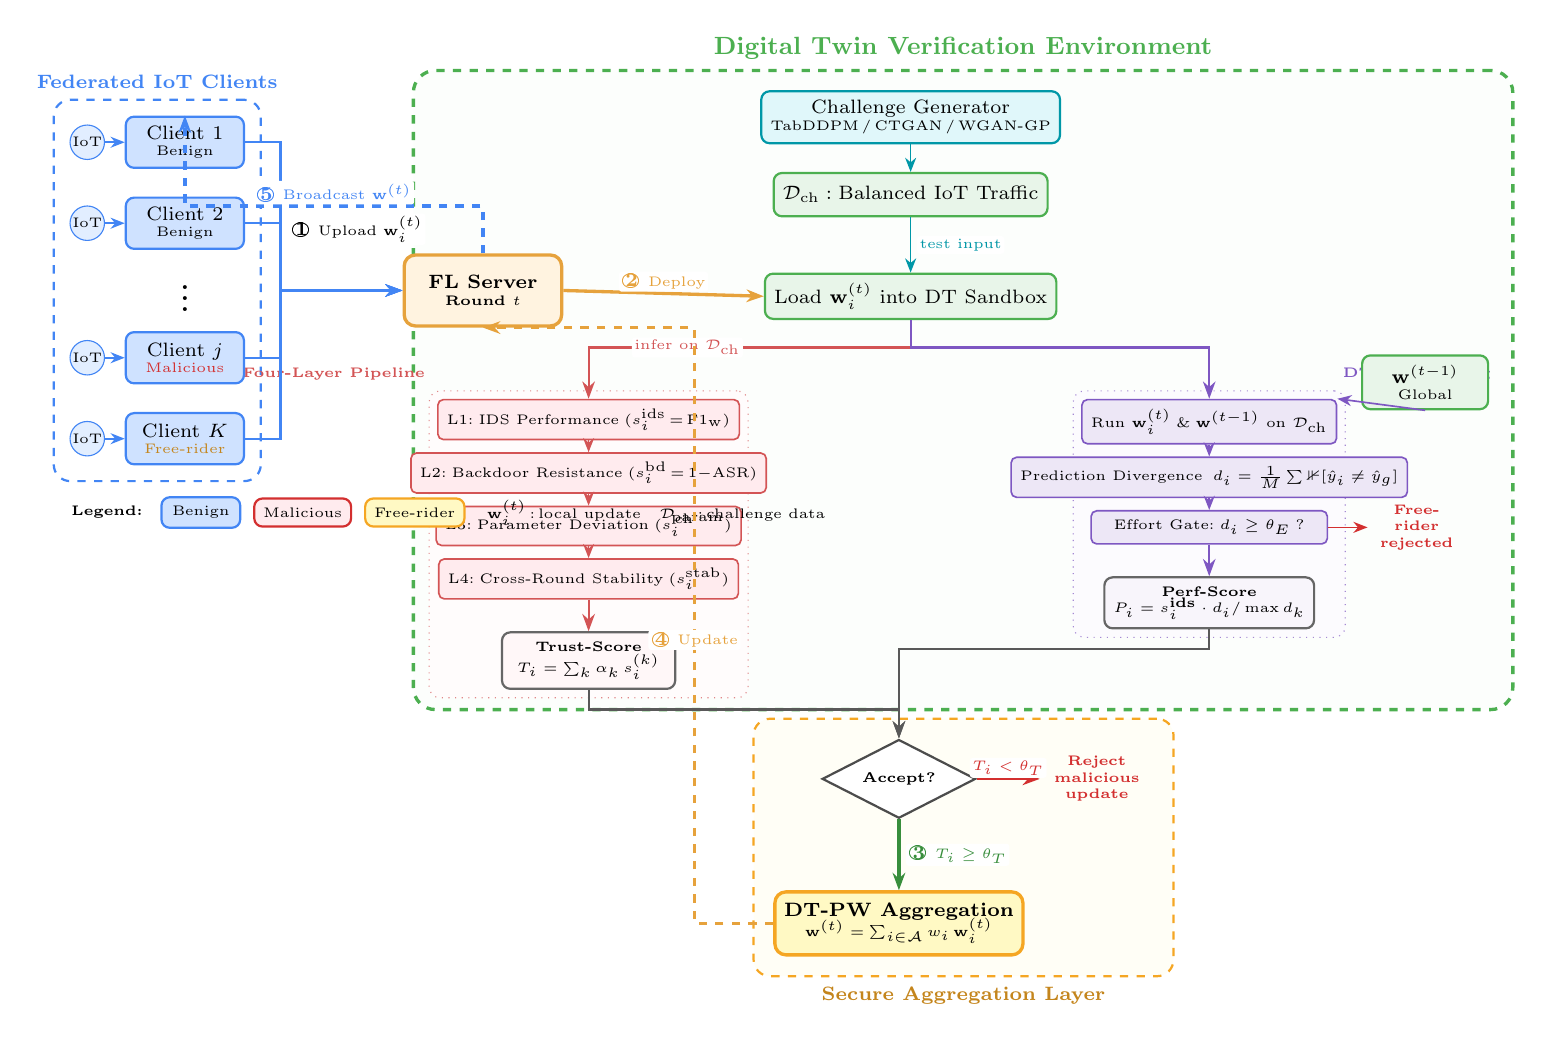
\begin{tikzpicture}[node distance=0.4cm and 0.6cm]

% ====================================================================
%  COLUMN 1 — IoT Clients (left side)
% ====================================================================
\node[clientbox] (c1) {Client 1\\[-2pt]{\tiny Benign}};
\node[clientbox, below=0.35cm of c1] (c2) {Client 2\\[-2pt]{\tiny Benign}};
\node[font=\small\bfseries, below=0.12cm of c2] (cdots) {$\vdots$};
\node[clientbox, below=0.12cm of cdots] (cm) {Client $j$\\[-2pt]{\tiny\color{rejectred} Malicious}};
\node[clientbox, below=0.35cm of cm] (cf) {Client $K$\\[-2pt]{\tiny\color{aggedge!80!black} Free-rider}};

% Small IoT icons
\foreach \c in {c1,c2,cm,cf}{
    \node[circle, draw=iotblue, fill=clientfill!60, inner sep=0.5pt,
          font=\fontsize{4}{4}\selectfont, left=0.25cm of \c] (iot\c) {IoT};
    \draw[thinarr=iotblue] (iot\c) -- (\c);
}

% ====================================================================
%  COLUMN 2 — FL Server
% ====================================================================
\node[serverbox, right=2cm of $(c2.east)!0.5!(cm.east)$] (srv) {FL Server\\[-2pt]{\tiny Round $t$}};

% Upload arrows
\foreach \c in {c1,c2,cm,cf}{
    \draw[arr=iotblue] (\c.east) -- ++(0.45,0) |- (srv);
}
\node[lbl, above left=0.1cm and -0.3cm of srv.north west]
    {\cmark{1} Upload $\mathbf{w}_i^{(t)}$};

% ====================================================================
%  COLUMN 3 — Digital Twin Verification Environment
% ====================================================================

% ── Challenge Generator (top)
\node[genbox, right=2.5cm of srv, yshift=2.2cm] (gen)
    {Challenge Generator\\[-2pt]{\tiny TabDDPM\,/\,CTGAN\,/\,WGAN-GP}};

% Challenge data
\node[dtnode, below=0.35cm of gen] (dch)
    {$\mathcal{D}_{\text{ch}}$\;:\;Balanced IoT Traffic};

% ── Deploy node
\node[dtnode, below=0.7cm of dch] (deploy)
    {Load $\mathbf{w}_i^{(t)}$ into DT Sandbox};

% Server -> Deploy
\draw[arr=serveredge, very thick] (srv.east) -- node[lbl, above] {\cmark{2} Deploy} (deploy.west);

% Gen -> D_ch -> Deploy
\draw[thinarr=genedge] (gen) -- (dch);
\draw[thinarr=genedge] (dch) -- node[lbl, right, xshift=2pt] {\tiny test input} (deploy);

% ── BRANCH LEFT: Four-Layer Verification Pipeline ──
\node[vnode, below left=1cm and 0.3cm of deploy] (v1)
    {L1:\;IDS Performance\;($s_i^{\text{ids}}$\,=\,F1$_{\text{w}}$)};
\node[vnode, below=0.15cm of v1] (v2)
    {L2:\;Backdoor Resistance\;($s_i^{\text{bd}}$\,=\,1$-$ASR)};
\node[vnode, below=0.15cm of v2] (v3)
    {L3:\;Parameter Deviation\;($s_i^{\text{param}}$)};
\node[vnode, below=0.15cm of v3] (v4)
    {L4:\;Cross-Round Stability\;($s_i^{\text{stab}}$)};

% Trust-Score
\node[scorebox, below=0.4cm of v4, fill=verifyfill!40] (tscore)
    {Trust-Score\\$T_i = \sum_k \alpha_k\, s_i^{(k)}$};

% Deploy -> V1
\draw[arr=verifyedge] (deploy.south) -- ++(0,-0.35) -| node[lbl, near start, left, xshift=-2pt] {\tiny infer on $\mathcal{D}_{\text{ch}}$} (v1.north);

% V chain
\draw[thinarr=verifyedge] (v1) -- (v2);
\draw[thinarr=verifyedge] (v2) -- (v3);
\draw[thinarr=verifyedge] (v3) -- (v4);
\draw[arr=verifyedge] (v4) -- (tscore);

% ── BRANCH RIGHT: DT-PW Contribution Scoring ──
\node[pwnode, below right=1cm and 0.3cm of deploy] (pw1)
    {Run $\mathbf{w}_i^{(t)}$\;\&\;$\mathbf{w}^{(t{-}1)}$ on $\mathcal{D}_{\text{ch}}$};
\node[pwnode, below=0.15cm of pw1] (pw2)
    {Prediction Divergence\;\;$d_i = \frac{1}{M}\sum \mathbb{1}[\hat{y}_i \neq \hat{y}_g]$};
\node[pwnode, below=0.15cm of pw2] (pw3)
    {Effort Gate:\;$d_i \geq \theta_E$\;?};
\node[scorebox, below=0.4cm of pw3, fill=dtpwfill!40] (pscore)
    {Perf-Score\\$P_i = s_i^{\text{ids}} \cdot d_i / \max d_k$};

% Global model reference
\node[dtnode, right=0.3cm of pw1, yshift=0.5cm, minimum width=1.6cm] (gref)
    {$\mathbf{w}^{(t{-}1)}$\\[-2pt]{\tiny Global}};

% Deploy -> PW1
\draw[arr=dtpwedge] (deploy.south) -- ++(0,-0.35) -| (pw1.north);

% Global -> PW1
\draw[thinarr=dtpwedge] (gref.south) -- (pw1.north east);

% PW chain
\draw[thinarr=dtpwedge] (pw1) -- (pw2);
\draw[thinarr=dtpwedge] (pw2) -- (pw3);
\draw[arr=dtpwedge] (pw3) -- (pscore);

% Free-rider reject from Effort Gate
\node[font=\tiny\color{rejectred}\bfseries, right=0.5cm of pw3, text width=1cm, align=center] (frlabel) {Free-rider\\rejected};
\draw[thinarr=rejectred] (pw3.east) -- (frlabel.west);

% ====================================================================
%  BOTTOM — Gate + Aggregation
% ====================================================================

% Decision gate
\node[gatediamond, below=1cm of $(tscore.south)!0.5!(pscore.south)$] (gate) {Accept?};

% Both scores -> Gate
\draw[arr] (tscore.south) -- ++(0,-0.25) -| (gate);
\draw[arr] (pscore.south) -- ++(0,-0.25) -| (gate);

% Reject path
\node[font=\tiny\color{rejectred}\bfseries, right=0.8cm of gate, text width=1.2cm, align=center] (rej)
    {Reject\\{\fontsize{4}{4}\selectfont malicious update}};
\draw[arr=rejectred] (gate.east) -- node[lbl, above] {\tiny $T_i < \theta_T$} (rej.west);

% Accept path -> Aggregation
\node[aggbox, below=0.9cm of gate] (agg)
    {DT-PW Aggregation\\[-2pt]{\tiny $\mathbf{w}^{(t)} = \sum_{i \in \mathcal{A}} w_i\,\mathbf{w}_i^{(t)}$}};
\draw[arr=acceptgreen, very thick] (gate.south) -- node[lbl, right, xshift=2pt] {\cmark{3} \tiny $T_i \geq \theta_T$} (agg.north);

% ====================================================================
%  FEEDBACK LOOP — Broadcast updated global model
% ====================================================================
\draw[darr=serveredge, very thick]
    (agg.west) -- ++(-1,0) |- node[lbl, near start, below, yshift=-1pt] {\cmark{4} Update} (srv.south);

\draw[darr=iotblue, very thick]
    (srv.north) -- ++(0,0.6) -| node[lbl, near start, above] {\cmark{5} Broadcast $\mathbf{w}^{(t)}$} (c1.north);

% ====================================================================
%  BACKGROUND BOXES
% ====================================================================
\begin{scope}[on background layer]
    % IoT Clients
    \node[draw=iotblue, thick, dashed, rounded corners=6pt,
          fit=(iotc1)(iotcf)(c1)(cf),
          inner sep=0.2cm,
          label={[font=\scriptsize\bfseries\color{iotblue}]above:Federated IoT Clients}] {};

    % Digital Twin
    \node[draw=dtedge, very thick, dashed, rounded corners=8pt,
          fill=dtfill!15,
          fit=(gen)(dch)(deploy)(v1)(v4)(tscore)(pw1)(pw3)(pscore)(gref)(frlabel),
          inner xsep=0.3cm, inner ysep=0.25cm,
          label={[font=\small\bfseries\color{dtedge}]above:Digital Twin Verification Environment}] {};

    % Four-Layer sub-region
    \node[draw=verifyedge!70, thin, dotted, rounded corners=4pt,
          fill=verifyfill!15,
          fit=(v1)(v4)(tscore),
          inner sep=0.1cm,
          label={[font=\tiny\bfseries\color{verifyedge}]above left:Four-Layer Pipeline}] {};

    % DT-PW sub-region
    \node[draw=dtpwedge!70, thin, dotted, rounded corners=4pt,
          fill=dtpwfill!15,
          fit=(pw1)(pw3)(pscore),
          inner sep=0.1cm,
          label={[font=\tiny\bfseries\color{dtpwedge}]above right:DT-PW Scoring}] {};

    % Aggregation
    \node[draw=aggedge, thick, dashed, rounded corners=6pt,
          fill=aggfill!15,
          fit=(gate)(agg)(rej),
          inner sep=0.25cm,
          label={[font=\scriptsize\bfseries\color{aggedge!80!black}]below:Secure Aggregation Layer}] {};
\end{scope}

% ====================================================================
%  LEGEND (bottom-left)
% ====================================================================
\node[font=\tiny\bfseries, anchor=north west] at ($(iotc1.west)+(-0.1,-4.5)$) (legtitle) {Legend:};
\node[clientbox, minimum width=1cm, minimum height=0.3cm, right=0.1cm of legtitle, anchor=west]
    (legben) {\tiny Benign};
\node[clientbox, minimum width=1cm, minimum height=0.3cm, fill=verifyfill,
      draw=rejectred, right=0.15cm of legben, anchor=west]
    (legmal) {\tiny Malicious};
\node[clientbox, minimum width=1cm, minimum height=0.3cm, fill=aggfill,
      draw=aggedge, right=0.15cm of legmal, anchor=west]
    (legfr) {\tiny Free-rider};
\node[font=\tiny, right=0.15cm of legfr, anchor=west]
    {$\mathbf{w}_i^{(t)}$\,:\,local update\quad$\mathcal{D}_{\text{ch}}$\,:\,challenge data};

\end{tikzpicture}
\end{document}
